\documentclass{article}

\usepackage{graphicx} % Required for the inclusion of images
\usepackage{adjustbox}
\usepackage{float}
\usepackage{textcomp,upquote,listings, color}
\usepackage{url}
\usepackage{booktabs}
 \definecolor{codegreen}{rgb}{0,0.6,0}
\definecolor{codegray}{rgb}{0.5,0.5,0.5}
\definecolor{codepurple}{rgb}{0.58,0,0.82}
\definecolor{backcolour}{rgb}{0.95,0.95,0.92}

\setlength\parindent{20pt} % Removes all indentation from paragraphs

\lstdefinestyle{mystyle}{
    backgroundcolor=\color{backcolour},   
    commentstyle=\color{codegreen},
    keywordstyle=\color{magenta},
    numberstyle=\tiny\color{codegray},
    stringstyle=\color{codepurple},
    basicstyle=\footnotesize,
    breakatwhitespace=false,         
    breaklines=true,                 
    captionpos=b,                    
    keepspaces=true,                 
    numbers=left,                    
    numbersep=5pt,                  
    showspaces=false,                
    showstringspaces=false,
    showtabs=false,                  
    tabsize=3
}
 
\lstset{style=mystyle}
\lstset{upquote=true}

%----------------------------------------------------------------------------------------
%	DOCUMENT INFORMATION
%----------------------------------------------------------------------------------------

\title{Citations Network Project\\ ADVANCED DATABASE SYSTEMS \\ADB - IT502} % Title

\author{Nguyen Hoang Minh - MITIU14005\\Chiem Thach Phat - MITIU14006} % Author name

\date{Fall 2014} % Date for the report

\begin{document}

\maketitle
\begin{center}
\begin{tabular}{l r}
Instructor: & Nguyen Hong Quang
\end{tabular}
\end{center}

%----------------------------------------------------------------------------------------
%	SECTION 1
%----------------------------------------------------------------------------------------

\section{General Terms}

This section describes terms used in this study.\\
CINAS : Citations Network Analysis\\
GDB : Graph Database\\
OM : Object-Mapping \\
ORM : Object-Relational Mapping \\
ODM : Object-Document Mapping \\
OGM : Object-Graph Mapping \\
RDBMS : Relational Database Management System \\
RDB : Relational Database\\
USPTO : United States Patent and Trademark Office\\

%----------------------------------------------------------------------------------------

\section{Conceptual Model (Analysis Task)}

We want to build a system that can store and analyze patents from USPTO as described in figure~\ref{fig:erd}. A patent contains an unique Publication number, Publication type, Application number, Publication date, Filling date, Priority date, Fee status (Paid or Free), Title, Length of grant (years), Classification and some of its contents include Abstract, Images, Description and Claims. A patent may or may not cite any other patents; and it may or may not be cited by other patents. A patent must be invented by at least one Inventor, be applied by only one Applicant, be assigned for at least one Assignee and be examined by at least one Examiner. The system will identify Inventor, Applicant, Assignee and Examiner by four attributes, which are their first name, last name, city and country.
\begin{figure}[h!]
\centering
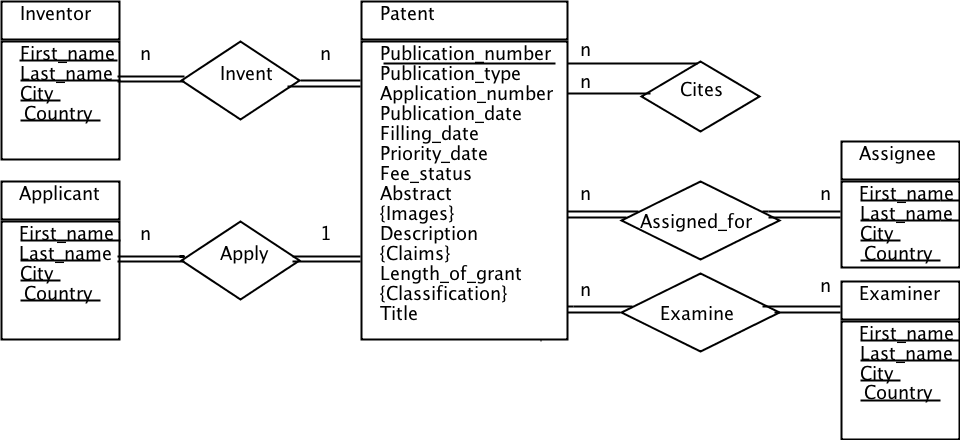
\includegraphics[width=\textwidth]{erd.png}
\caption{ PatentDB Conceptual Model} \label{fig:erd}
\end{figure}\par
Due to limited resources, instead of implementing the complete system, we chose the simple modelling to convey the operations of CINAS. The database is called PatentDB which has only two entities, inventor and patent. The relationship between entities and its attribute are illustrated in figure~\ref{fig:conceptual}.\\~\\
\begin{figure}[h!]
\centering
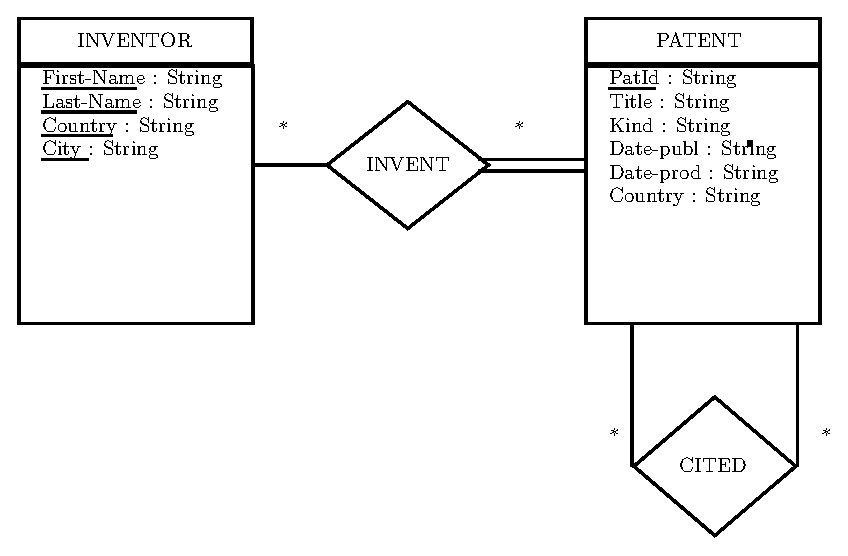
\includegraphics[width=\textwidth]{conceptual_model.eps}
\caption{ Demo Conceptual Model} \label{fig:conceptual}
\end{figure}\par~\\
Rules are simple as follow:
\begin{itemize}
  \item An inventor may invent many patents and many inventors can work on the same one
  \item A patent might be cited by other patents or may refer to many patents
\end{itemize}

%----------------------------------------------------------------------------------------

\section{Logical Model (Design Task)}
\subsection{Mapping to Graph Logical Model (Neo4j)}
In Neo4J, logical model can be represented by nodes with relationships as in figure~\ref{fig:neo4j}.\\
The system has:
\begin{itemize}
\item Two types of Node: \textbf{Patent} and \textbf{Inventor}
\item \textbf{Patent} has a relationship named \textbf{CITEDBY} with \textbf{other Patents}
\item \textbf{Inventor} has a relationship \textbf{INVENT} with \textbf{Patents}
\item Node also has \textbf{Properties}, such as \textbf{Inventor has first\_name} and \textbf{Patent has publication\_number}
\end {itemize}

\begin{figure}[h!]
\centering
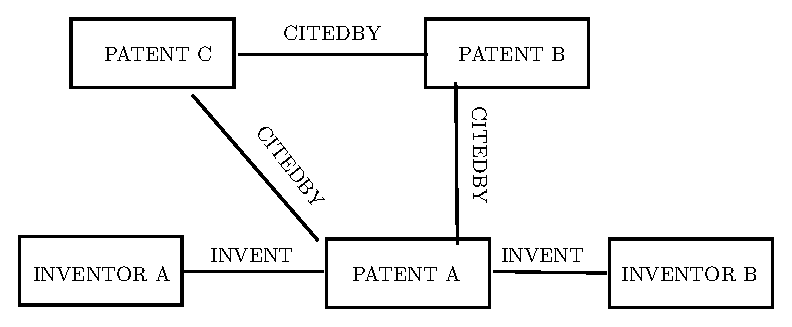
\includegraphics[width=80mm,scale=10]{neo4jgraph.eps}
\caption{ PatentDB Conceptual Model} \label{fig:neo4j}
\end{figure}

\subsection{Mapping to Document-oriented Logical Model (MongoDB)}
With MongoDB, related data is embedded in a single structure or document. These schemas are generally known as "denormalized" models, and take advantage of MongoDB's rich documents. Consider the following schema:
\begin{lstlisting}[caption=Document-oriented schema]
patent_schema = {
    kind : string, 
    date-published : string, 
    number-of-claims : integer, 
    country : string, 
    patid : string,
    main-classification : string,
    title : string,
    app-number : string, 
    citations : [ { patid : string }, { patid : string }]
    date-produced : string, 
    inventors:[
    	{city:string, last-name:string, country:string, first-name:string},
    	{city:string, last-name:string, country:string, first-name:string}
     ]       
}

inventor_schema={
    city : string, 
    last-name : string, 
    country : string, 
    first-name : string
}
\end{lstlisting}

As we design, the \textbf{patent\_schema} is \textbf{embedded with} the \textbf{inventor\_schema in inventors} key, as described from line 12 to 15 in listing 1.\par
In general, embedding provides better performance for read operations, as well as the ability to request and retrieve related data in a single database operation. Embedded data models make it possible to update related data in a single atomic write operation.\par
However, embedding related data in documents may lead to situations where documents grow after creation. Document growth can impact write performance and lead to data fragmentation. We would use reference for patent's citations. However, client-side applications must issue follow-up queries to resolve the references.

%----------------------------------------------------------------------------------------

\section{Data Storage}
In this section, we will describe each component of CINAS in detail and also discuss design methodology. Fully written in Python, CINAS consists of 2 main modules:
\begin{enumerate}
 \item Firstly, XML Parser Module \textbf{parses the input XML file into JSON format}.
 \item DB Client would then \textbf{load JSON format files to populate it into Database}.
\end{enumerate}
REST services are provided by external resources.
\begin{figure}[H]
\centering
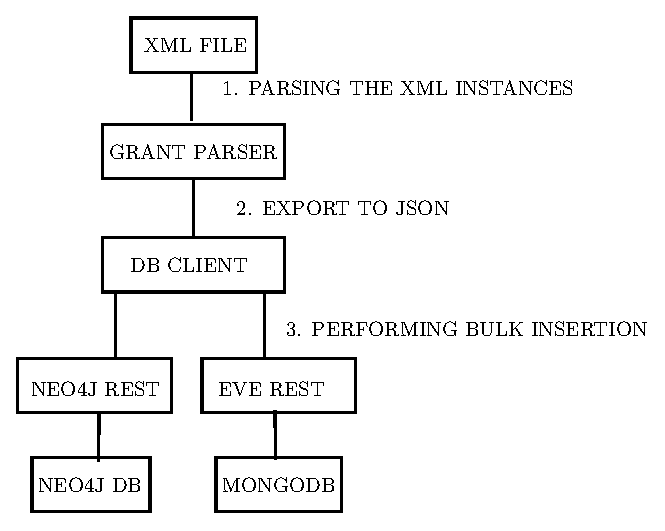
\includegraphics[width=80mm,scale=0.1]{cinasstruct.eps}
\caption{ CINAS ARCHITECTURE}
\end{figure}
\subsection{XML Parser Module}
There are \textbf{two approaches in designing XML Parser}. Either one may choose \textbf{DOM} method, which load the entire file onto memory using ElementTree, or line by line processing by \textbf{SAX}. Even though the \textbf{former method is remarkably simpler and faster, it is susceptible to memory consumption}. As data grows big, implementing parser using DOM method is not plausible. Fortunately, \textbf{the latter is well suit for parsing big data by design and thus, will be implemented in CINAS}.

\begin{figure}[H]
\centering
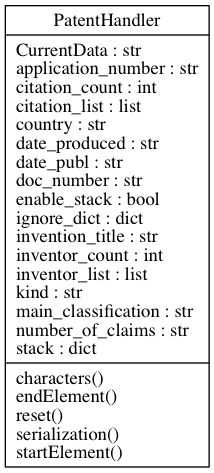
\includegraphics[width=40mm,scale=10]{handler.png}
\caption{Patent Handler Class Diagram} \label{fig:handler}
\end{figure}

The core of Grant Parser script is PatentHandler class, class diagram of it is shown in figure~\ref{fig:handler}. It mainly used to hold data that parsed from each XML instance. Since SAX Parser only read XML line by line, it's reasonable to keep track of processing tag using stack. In brief, Grant Parser currently works following this procedure:
\begin{enumerate}
 \item Load XML file and break it down into separated XML instances
 \item Parse each XML instance into patent handler. For each tag with nested tags, enable stack to store adjacent data.
 \item Tags that are explicitly defines in ignore list will be left out during parsing. Upon completion, reset the patent handler for new instance
 \item Finally, an option to export the entire file to JSON format is available if chosen.
\end{enumerate}

An implementation using DOM tree is also documented solely for benchmark's comparison and thus, detailed explanations are beyond the scope of this study.

\subsection{DB Client Module}
Instead of using OM for particular database, we chose to \textbf{deploy REST services as mean of communication with our backends}. It is complicated to wrap OM around another OM, but it is simple to wrap data around HTTP response and request before forwarding. Therefore this approach provides more scalable solution than OM. Despite the fact that \textbf{this approach might limit the performance speed, it is worth a trade-off for being more extendable}. The figure~\ref{fig:db_client} illustrates class diagram of our DB Client module.

\begin{figure}[H]
\centering
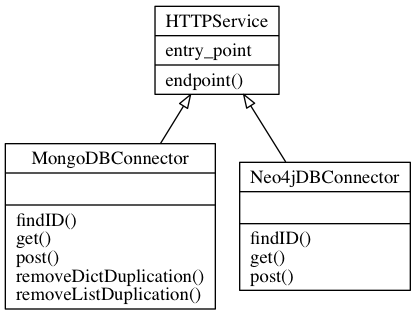
\includegraphics[width=80mm,scale=10]{db_client.png}
\caption{ DB Client Class Diagram \label{fig:db_client}}
\end{figure}

The idea is to create an abstract layer to hide the presence of multi-databases systems. Instead of choosing ODM for MongoDB or OGM for Neo4J, we created an data layers to a enhance the transparency. For example, to issue a POST request to whatever the backend is, developers currently only need to concern the differences between resources and query format (commonly JSON). The complexity underlying will be handled by each corresponding connectors. As can be seen from figure \ref{fig:db_client}, \textbf{all the fundamental HTTP methods are implemented in HTTPService}. MongoDBConnector and Neo4jDBConnector inherit private methods from its parent. 

It's important to note that we need to handle with cares for MongoDB as it's susceptible to data redundancy and inconsistency due to being no schema DB. In addition, MongoDB requires an object ID to make a legitimate references. In specific, for a patent to make references, it should store the objectID of patent instead of proposed patent ID. From our opinions, we think this is unnecessary and generate extra workload for conversions. Hence, we \textbf{use embedded to represent the relationships between patent}. 

Regarding the duplication in MongoDB, considering this case where patent 08852195 actually refer to WO2005/069809 twice at line 329 and line 330\footnote{http://www.directorypatent.com/US/08852195.html}, it's inevitable that we might have data redundancies to some extents. Even though it's more acceptable to treat them as one entity, we would consider it in our next stage of implementation due to time constraint.

The procedure of \textbf{POST in MongoDB} is:
\begin{enumerate}
 \item Load all data from JSON file
 \item Construct list of citations from group of patent
 \item Validate uniqueness within the list. When we insert using bulk insertion, 3 patents might references the same patent and this will culminate in data duplication in DB. We can not overlook this problem.
 \item Appending statements into query. Then, perform 1st POST these citations 
 \item If the uniqueness is violated, the response code from EVE server will determine the next step. If error response with duplicates found, we remove it from the list and resend it again.
 \item Finally, we perform an overwrite PUT for any individual patent. This step must be linearly execute to guarantee that all the dummy patents, which are created using citations, will be updated with information.
\end{enumerate}

The procedure of \textbf{POST in Neo4J is much more simpler}, since Neo4J has an overwrite operation called "MERGE",which will create or merge properties to existing node, and allow developers to execute it through Cypher endpoint. Therefore, it reduces the need for extra validation:
\begin{enumerate}
 \item Load all data from JSON file
 \item Construct list of citations from group of patent
 \item Appending statements into query. Then, perform POST these citations 
 \item Finally, we perform another POST for list of patents.
\end{enumerate}

%----------------------------------------------------------------------------------------

\section{Results (End-User Functionalities Task)}
Contemporarily, CINAS has processed up to 110343 so-called patents. Table~\ref{table:summarize} shows the summarized statistic of patent database.
\begin{table}[!h]
\begin{center}
\begin{tabular}{|c|c|l|} \hline
 &Number of Documents\\ \hline
 Duplicated Citations&347 \\ \hline
Patents&3000 \\ \hline
Citations&106996 \\ \hline
Total & 110343\\ \hline
\end{tabular}
\end{center}
\caption{Summarize Table} \label{table:summarize}
\end{table}

\begin{table*}[h!]
\begin{adjustbox}{max width=\textwidth}
\begin{tabular}{|c|c|l|} \hline
 Class & Descriptions \\ \hline
D99 & MISCELLANEOUS \\ \hline
D34 & MATERIAL OR ARTICLE HANDLING EQUIPMENT\\ \hline
D32 & WASHING, CLEANING, OR DRYING MACHINE\\ \hline
D30 & ANIMAL HUSBANDRY\\ \hline
D29 & EQUIPMENT FOR SAFETY, PROTECTION, AND RESCUE (1)\\ \hline
D28 & COSMETIC PRODUCTS AND TOILET ARTICLES\\ \hline
D26 & LIGHTING\\ \hline
D25 & BUILDING UNITS AND CONSTRUCTION ELEMENTS\\ \hline
D24 & MEDICAL AND LABORATORY EQUIPMENT\\ \hline
D23 & ENVIRONMENTAL HEATING AND COOLING; FLUID HANDLING AND SANITARY EQUIPMENT\\ \hline
D21 & GAMES, TOYS, AND SPORTS EQUIPMENT\\ \hline
D20 & SALES AND ADVERTISING EQUIPMENT\\ \hline
D19 & OFFICE SUPPLIES, ARTISTS AND TEACHERS MATERIALS\\ \hline
D17 & MUSICAL INSTRUMENTS\\ \hline
D16 & PHOTOGRAPHY AND OPTICAL EQUIPMENT\\ \hline
D15 & MACHINES NOT ELSEWHERE SPECIFIED\\ \hline
D14 & RECORDING, COMMUNICATION, OR INFORMATION RETRIEVAL EQUIPMENT\\ \hline
D13 & EQUIPMENT FOR PRODUCTION, DISTRIBUTION, OR TRANSFORMATION OF ENERGY\\ \hline
D12 & TRANSPORTATION\\ \hline
D11 & JEWELRY, SYMBOLIC INSIGNIA, AND ORNAMENTS\\ \hline
D10 & MEASURING, TESTING OR SIGNALING INSTRUMENTS\\ \hline
D9 & PACKAGES AND CONTAINERS FOR GOODS\\ \hline
D8& TOOLS AND HARDWARE \\ \hline
D7& EQUIPMENT FOR PREPARING OR SERVING FOOD OR DRINK NOT ELSEWHERE SPECIFIED \\ \hline
D6 & FURNISHINGS\\ \hline
D5 & TEXTILE OR PAPER YARD GOODS; SHEET MATERIAL\\ \hline
D4 & BRUSHWARE\\ \hline
D3 & TRAVEL GOODS AND PERSONAL BELONGINGS\\ \hline
D2 & APPAREL AND HABERDASERY\\ \hline
D1 & EDIBLE PRODUCTS\\ \hline
\end{tabular}
\end{adjustbox}
\centering
\caption{USPTO - Classification Table} \label{tab:class}
\end{table*}

\begin{figure}[H]
\centering
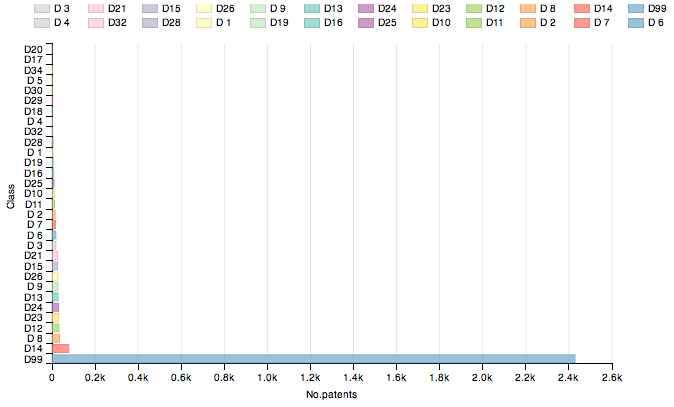
\includegraphics[width=\textwidth]{rplot-classification.png}
\caption{ Patent Classification October 2014 }\label{fig:rplot}
\end{figure}

From figure~\ref{fig:rplot} and table~\ref{tab:class}, it is immediately striking that inventions for MISCELLANEOUS (D99) industry were blossomed in October 2014. In specific, nearly 2500 granted patents (accounted for nearly 83\%) makes non-trivial goods production industry become the most popular topic among the invention community. In addition, this might signal a competitive field for any inventors that shall want to take part in. On the opposite, classification that are larger than 20 were recorded at lowest level, except for the case of  MEDICAL AND LABORATORY EQUIPMENT (D24), ENVIRONMENTAL HEATING AND COOLING; FLUID HANDLING AND SANITARY EQUIPMENT (D23) and LIGHTING(26) where number of inventions are relatively close to those in range of 1x (approx. 100). In general, involving in these fields might be less competitive than the others. Even though coming in second place of the ladder, RECORDING, COMMUNICATION, OR INFORMATION RETRIEVAL EQUIPMENT's inventions (D14) are accounted for merely 6.66\%, in other words, 15 times smaller than the dominant D99. Interestingly, this also indicates the need for more robust information retrieval system is significant and thus, was main motivation for this study. Following D14 closely was TOOLS AND HARDWARE (D8) which received 150 attentions. Finally, we  also witness the insignificant presence of inventions in various class among 1x and 0x. As promised, statistics and bar chart was computed and generated using R.

\subsection{Citations Network}

We also demonstrate citations network on 500 patents instead of 3000 patents due to memory constrain on personal computer. A full view of network consists of inventors, patents, citations and their links are shown in figure~\ref{fig:citation}. 
\begin{figure}[H]
\centering
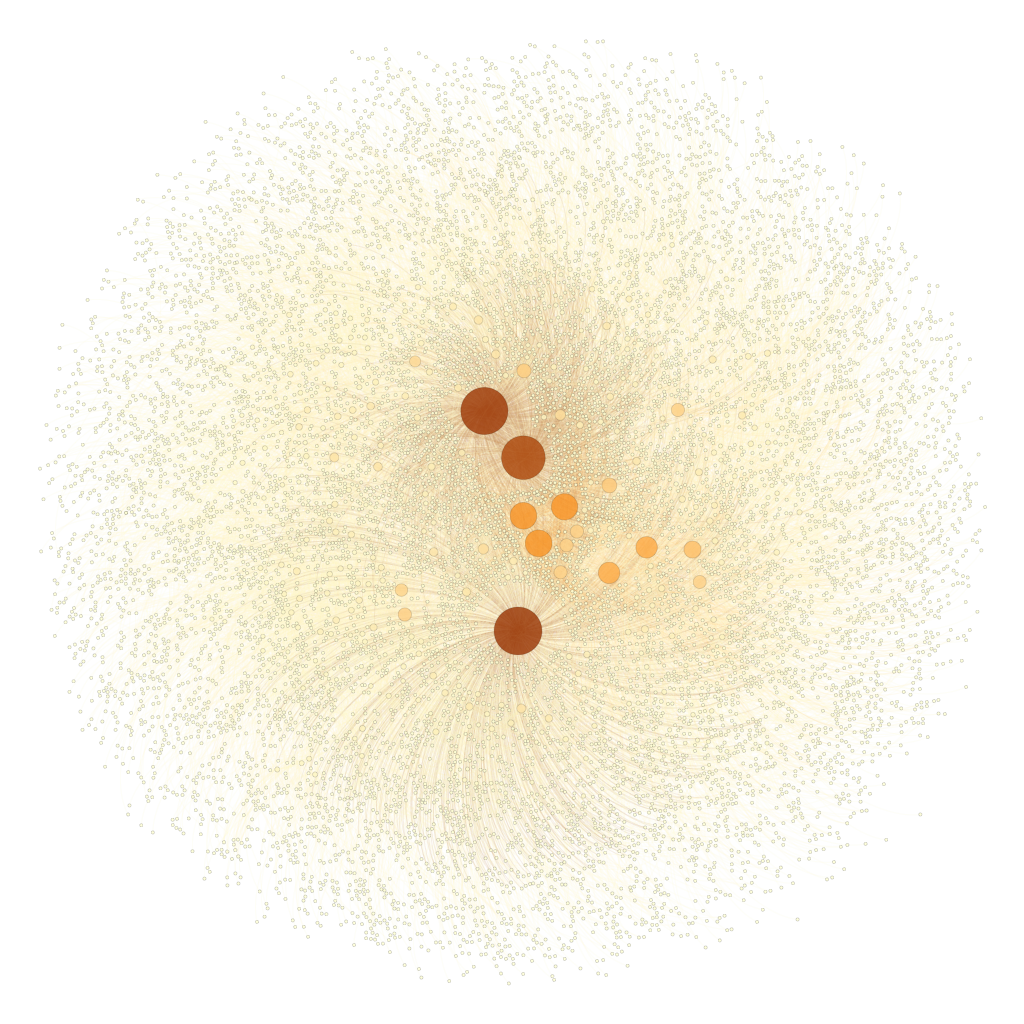
\includegraphics[width=70mm]{citation.png}
\caption{ Patents and Citations October 2014 }\label{fig:citation}
\end{figure}

\begin{figure}[H]
\centering
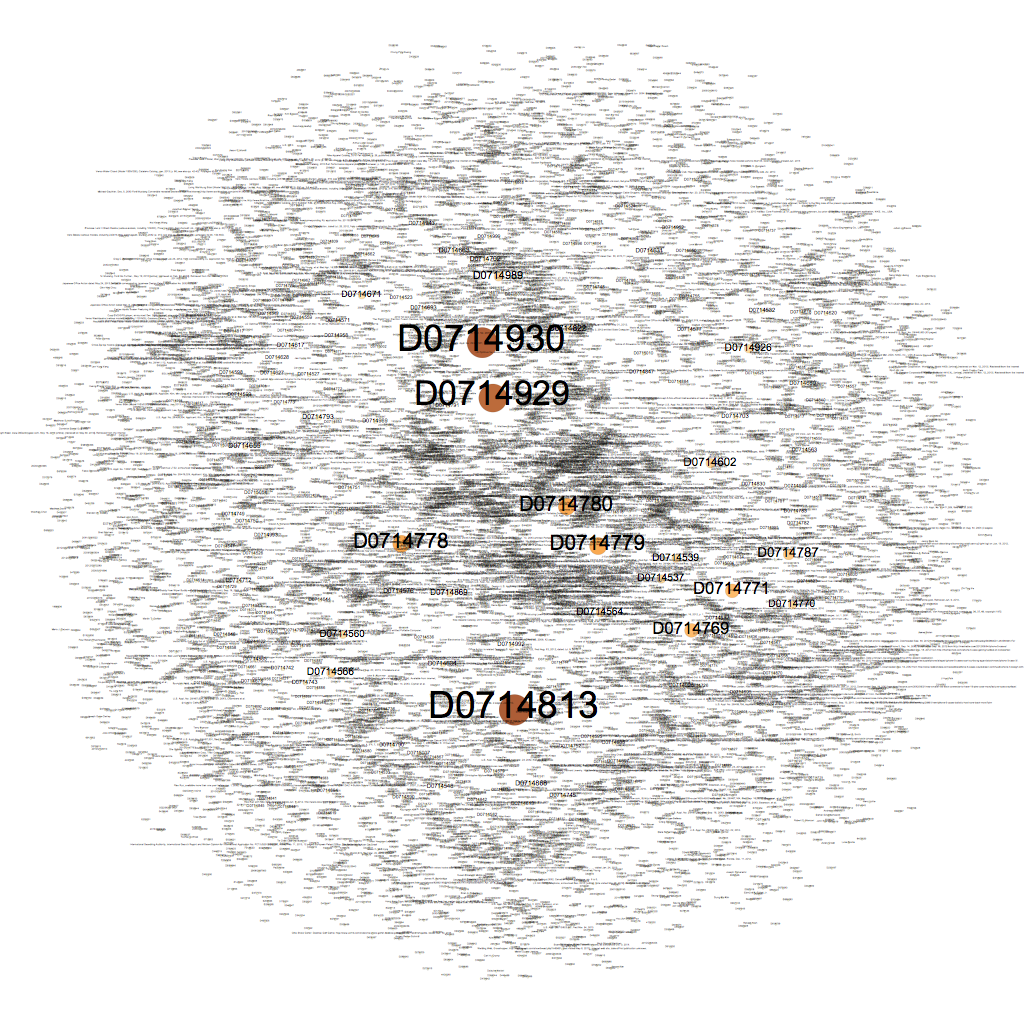
\includegraphics[width=80mm]{citation-label.png}
\caption{ Citations Network October 2014 }\label{fig:citationlabel}
\end{figure}

In this figure, using Gephi as visualization tool to enhance the spatialization within the network, we applied the force-directed layout Fruchterman Reingold to scatter out the node\footnote{http://en.wikipedia.org/wiki/Force\-directed\_graph\_drawing} and Force Atlas to distribute nodes without overlapping\footnote{http://webatlas.fr/tempshare/ForceAtlas2\_Paper.pdf}. Specifically, Bigger nodes will be gather at the central of the graph while nodes with least connections are pushed to the rear area. A closer look at citations network can be observed from figure~\ref{fig:citationlabel}. In particular, we applied ranking by connected components to distinguish group of nodes which have largest number of connections.\par
Ranking by connected components gives us the importances of particular node since not only many inventors connect to it, but also do many inventions actual refer to it as a fundamental foundation.  
\begin{table}[H]
\centering
\begin{tabular}{|c|c|c|c|}  \hline
 ID&Title&No.citations&Class\\ \hline
 D0714930&Reservoir.for.water.flosser&495&D24\\ \hline
D0714929&Base.for.water.flosser&457 &D24\\ \hline
D0714813&Electronic.camera&517&D14 \\ \hline
\end{tabular}
\caption{Most connected components patents information}\label{tab:component}
\end{table}
Table~\ref{tab:component} shows the information regarding group of most-connected nodes from the graph. Unfortunately, All of them are recently published and thus, we can not observe the case where patent from the past was referred by many patents from this figure.
In figure~\ref{fig:endcitation}, the edges of the network reflect patents or inventors that are connected to only one node of the graph. Following the connected-components ranking algorithm, we might deduce that they are lack of popularity and feasible knowledge.
 \begin{figure}[H]
\centering
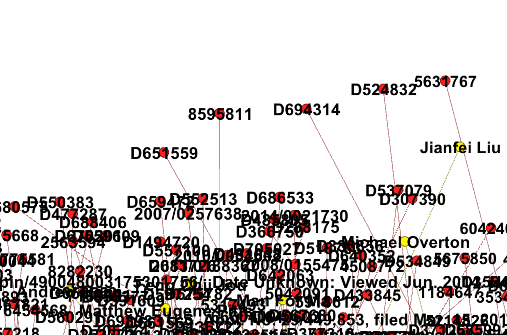
\includegraphics[width=80mm]{endcitation.png}
\caption{ Citations Network Edge October 2014 }\label{fig:endcitation}
\end{figure}

\subsection{Inventors Maps}
To measure the activity of inventors community, we classify them based on their regions in figure~\ref{fig:map}. It's not surprising to witness the outstanding in the field of North America since it's their nation to begin with. However, it's interesting to see that US patents industry also attracts the numerous inventors from different parts of the world, including Asian and Australian. Besides, Russia, despite being second polar of the world in term of economy and currently has oil dispute with American, has no inventors take part in. Overall, the figure might indicate the inventing opportunities in US patent industry from the perspective of the outsiders.
 \begin{figure}[H]
\centering
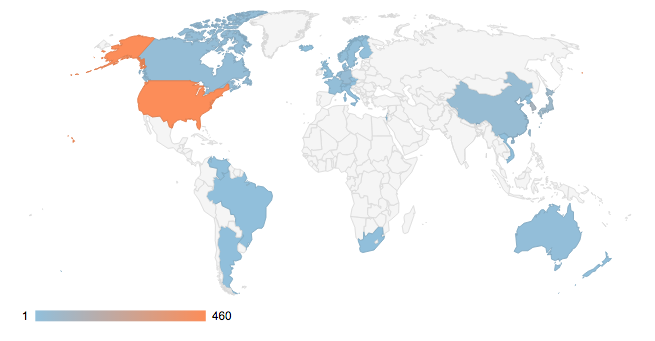
\includegraphics[width=90mm]{inventor-map.png}
\caption{ Geographic of inventors October 2014 }\label{fig:map}
\end{figure}

 \subsection{Benchmark Neo4J and MongoDB}
 \begin{table*}[H]
 \centering

\begin{tabular}{lllllll}
\toprule 
    Patents & \multicolumn{2}{c}{Parsing} &\multicolumn{2}{c}{Insertion with Duplication}\\

    & SAX & DOM 
    & Neo4J-REST & MongoDB-REST & Neo4J-OGM\\
    \midrule
    $50 + 1224$     & 0.96s & 0.05s  &248.44 & 15.64 & 58.488 \\
    $100 + 2306$  & 1.47s & 0.09s &448.65 & 30.88 & 107.177\\
    $200 + 4439$  & 2.68s & 0.18s&974.57 & 87.55 & 218.85\\
    $300 + 7834$  & 4.42s& 0.29s&1476.65 & 159.04 & 348.68\\
    $400 + 9313$  & 6.48s & 0.38s&2942.61 & 213.21 & 467.74\\
    $500 + 12016$  & 6.99s& 0.53s &2780.16 & 287.58 & 610.102\\
    \bottomrule
\end{tabular}
\caption{Write performance of CINAS}
\end{table*}

 We perform the time measurements on 500 patents with total of 12016 citations. DOM and OGM are tested on personal computer that can actually handle the entire XML files of 500MB while the rests are tested on limited resources host. The following cases are taken into consideration:
 \begin{itemize}
 \item  Parsing XML using DOM
 \item Parsing XML using SAX
 \item Insertion of Neo4J throught built-in REST server
 \item Insertion of MongoDB throught Eve REST server
 \item Insertion of Neo4J throught OGM
\end{itemize}
 
All the statistics are presented in table 8, its corresponding graph is figure \ref{fig:benchmark}. Overall, the trade-off between SAX and DOM, OGM and REST are clearly visualized. In particular, as SAX has to process data line by line, it's inevitably slower than DOM which load the whole file onto the memory. In addition, OGM is faster than REST in term of performance, but the simplicity of REST is worth the trade-off to develop more sustainable solutions. As can be seen from the graph, insertions with Neo4J are relatively time-consuming as nodes together with links need to be created. Futhermore, the graph is exponentially increased so Neo4J alone will not suitable solution for big data. On the opposite, MongoDB has higher write performance since everything is stored without constrains and relationships. The drawback of MongoDB is that end-client has to implement the references between each document, enforce data validations and thus, require more works load on the client side. 
 
 \begin{figure}[H]
\centering
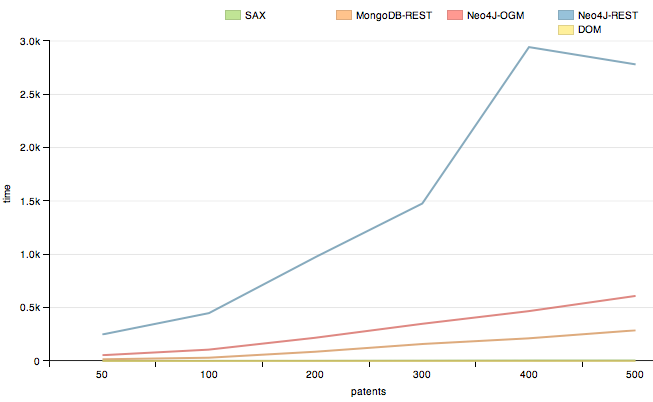
\includegraphics[width=\textwidth]{line.png}
\caption{CINAS Benchmark} \label{fig:benchmark}
\end{figure}

\section{Lessons Learned}
CINAS initially aims to provide more flexible and scalable solution for big patent data. Similar to other systems, the process of analyzing patents following CINAS are explained as follow:

\begin{itemize}
\item Extracting valuable information
\item Inserting into database
\item Exporting the information
\end{itemize}

It's important to note that CINAS is designed to be DBMS-independent. Specifically, the framework has special connectors working as drivers to different databases and thus, can fully take advantages of crossing-database's characteristics. For example, \textbf{to analyze a citation network in which contains nested relationships and thousand of nodes,  Neo4J is far superior than RDBMS}. Nonetheless, \textbf{Neo4J is remarkably slow when it comes to big data} as it stores additional attributes in the relationships between nodes and presents more complicated relationships between each node in comparison to RDBMS. Another example is \textbf{to analyze text-based field where MongoDB would take primary place because it has no schema enforced on data}. No schema would also mean no joining cost in term of relational and hence, provide more speed. 

In this study, we present the method of obtaining citation network using Neo4j as back-end. Furthermore, we also show how valuable data can be extracted from MongoDB. The dramatical trade-off of this approach is that it would cost more memories, load-balance to maintain two different DBMS system within one host and hence, reducing overall speed. Having thought of that, we implemented CINAS using RESTful APIs to partially address those issues, we also compare the pros and cons with the ORM approach for references in implementation section. Even though it cannot overcome the speed of using ORM with direct-connection to the storage, it's worth mentioned in term of scalability.

\subsection{Neo4j}
Graph Database differs from RDB in the sense that a node itself is a "thing", not a table that holds many records. This provides a level of flexibility to represent data closer to the real world entity. Considering the following example where GDB overwhelms our traditional RDB, that's in a citation networks a patent is cited by many patents. Traditionally, RDB would maintain only single table, named Patent, with each record has an additional column to store foreign key. However, the fact that many patents can cite a single patent and a patent can be referred by many patents would leave us an M-to-N relationship and require a creation of second table. Suppose citations are limited to 1000 patents, which means cited patents and patents are reachable within our database, and each patent can refer up to 1000 patents. Clearly, 1000000 records should be stored inside our second table. Therefore, representing such a nested relationship with tabular system is not a scalable practice since we have more than millions of patents. The above problem can be addressed with 1000 nodes and 2000 relationship in GDB, this is much similar to what we usually think.

An additional important feature in GDB is relationship's weight, this offers more accurate ways to determine the relationship between each entity. 

\subsection{MongoDB}
MongoDB  is an open-source document database, and the leading NoSQL database. MongoDB deploys BSON as an primary data representation and therefore improve speed of traverse through JSON file. BSON, short for Binary JSON, is the binary-encoded version of JSON-like documents. In other words, it adds extensions for data types such as integer or date that are not part of JSON specification. JSON is a self-describing, human readable data format. Originally designed for lightweight exchanges between browser and server, it has become widely accepted for many types of applications. JSON documents are particularly useful for data management for several reasons. A JSON document is composed of a set of fields which are themselves key-value pairs. This means each JSON document carries its own human readable schema design with it wherever it goes, allowing the documents to easily move between database and client applications without losing their meaning. Detailed explanations for JSON and BSON will not be discussed in this study.

A record in MongoDB is a document, which is a data structure composed of field and value pairs. MongoDB documents are similar to JSON objects. The values of fields may include other documents, arrays, and arrays of documents. The advantages of using documents are:
\begin{itemize}
\item Documents (i.e. objects) can be defined with native data types that can be seen in many programming languages. E.x: Date, String, Integer
\item Embedded documents and arrays reduce need for expensive joins.
\item Dynamic schema supports fluent polymorphism.
\end{itemize}

\subsubsection{Downfall of Normalization }
This example was taken from Brian's blog\footnote{http://blog.mongodb.org/post/72874267152/transitioning-from-relational-databases-to-mongodb} to explain the drawbacks of normalization approach, we also change the data to patent data to illustrate similar problems can be faced in process of designing CINAS . The immediate and fundamental difference between MongoDB and an RDBMS is the underlying data model. A relational database structures data into tables and rows, while MongoDB structures data into collections of JSON documents. The ability to support arrays is an especially helpful feature. Consider the complexity of supporting a repeating group in a properly normalized table structure. To represent the same data object in a single table row would like like this:
\begin{table}[H]
\begin{tabular}{|c|c|l|} \hline
PatentID&Title&Classification\\ \hline
1& "Snack"& "D1, D2, D3"\\ \hline
\end{tabular}
\centering
\caption{Patent Table}
\end{table}
Aggregation and updating specific classification for a comma separated list might pose serious problems and extra works. The first normalization was designed to avoid such problems by dividing each class into different records.

\begin{table}[H]
\begin{tabular}{|c|c|l|} \hline
PatentID&Title&Classification\\ \hline
1& "Snack"& "D1"\\ \hline
1& "Snack"& "D2"\\ \hline
1& "Snack"& "D3"\\ \hline
\end{tabular}
\centering
\caption{1st Normalized Patent Table}
\end{table}

We create a data redundancies that make us susceptible to anomalies. An example is to issue update command using SQL query :

\begin{lstlisting}[caption=Json Example]
UPDATE Patent 

SET Title = "New Snack"  

WHERE PatentID = 1 

AND Classification = "D1"
\end{lstlisting}

\begin{table}[H]
\begin{tabular}{|c|c|l|} \hline
PatentID&Title&Classification\\ \hline
1& "New Snack"& "D1"\\ \hline
1& "Snack"& "D2"\\ \hline
1& "Snack"& "D3"\\ \hline
\end{tabular}
\centering
\caption{1st Normalized Patent Table}
\end{table}

This happens because the table fail to qualify a 2nd Normalization Form. Classification is not functionally dependent on Title since there are three titles with different classes. Hence, we need to normalize data into 2 separated tables.

\begin{table}[H]
\centering
\begin{tabular}{|c|c|l|} \hline
PatentID&Title\\ \hline
1& "Snack"\\ \hline
\end{tabular}

\begin{tabular}{|c|c|l|} \hline
PatentID&Classification\\ \hline
1& "D1"\\ \hline
1& "D2"\\ \hline
1& "D3"\\ \hline
\end{tabular}
\centering

\centering
\caption{2nd Normalized Patent Tables}
\end{table}

This structure prevents the anomaly, but introduces a new set of problems. The new schema has become much more complex, and we have lost any semantic understanding of stored objects. By adhering to these two normal forms, we've also entered the realm of cross-table joins and the need to enforce ACID transactions across multiple tables. The enforcement of referential integrity in multi-row, multi-table operations will require concurrency controls, increasing overhead and affecting performance.

MongoDB avoids these complications through the use of a document data model. The JSON document forms a more natural representation on the data than the normalized schema. It achieved this by allowing the embedding of related data via arrays and sub-documents within a single document - thus eliminating the need for JOINs, referential integrity and multi-record ACID transactions.

\begin{lstlisting}[caption=Json Example]
{
	{
	"_id" : ObjectId("528ba7691738025d11aab772"),
	"patid" : 1,
	"title": "Snack",
	"classification" : ["D1", "D2", "D3"]
	}
}
\end{lstlisting}

\subsection{OM and REST services}

\textbf{Object Mapping} is an layer over database to assist querying and managing data using an object paradigm. The \textbf{pros} of this method is that it hides the database query language syntax away from logic code. Following this manner, data models are gathered in one place and it's easier to update, maintain and reuse the code. Every databases have its different mapping methodology. For example, relational database will need object-relational-mapping while object-document mapping serves as driver between web applications with document-oriented database. The \textbf{drawback} of using OM is that OM tools generally stem from the high level of abstraction obscuring what is actually happening in the implementation code. Also, heavy reliance on OM software has been reported as a major factor in producing poorly designed databases. Furthermore, as we stated CINAS is database-indepedent, it's better to exchange data over more popular format such as JSON instead of binding to a specific database's language. Last but not least, OM does not provide neither enhanced security services as it has its own connection to the database, nor load-balancing. This would leave more works on the database's side.

\textbf{REST}, for REpresentational State Transfer, is a simple stateless architecture generally running over HTTP. REST has become the norm in past decades as the majority of developers would prefer this scalable solution\footnote{http://www.theserverside.com/feature/Why-developers-demand-resource-based-RESTful-APIs}.

We agree the \textbf{boons of REST services} over our CINAS which are described comprehensively in Swaroop Chitlur's blog\footnote{http://www.swaroopch.com/2013/04/18/database-as-rest-api/}:
\begin{itemize}
\item It's simpler in comparison to OM as it only uses GET, PUT, POST, DELETE and PATCH to communicate with the web services.
\item  Switching some data from Neo4J to MongoDB or sharding in MongoDB, etc. could be hidden as internals of this layer. This copes well with our requirements for database-independence.
\item Providing middle layer would also enhance rate-limiting, monitoring and scalability - and Database's memory leaks, etc. would not affect other parts of the system.
\end{itemize}

Despite having favors for REST, the services are generally \textbf{suffer from performance} as it wraps data through an additional layer and also provide an abstraction over databases.

\subsection{Gephi}
Unfortunately, \textbf{Neo4j visual browser only supports up to 1000 rows}\footnote{http://stackoverflow.com/questions/26031795/resultset-too-large-over-1000-rows-in-neo4j-browser} and the \textbf{performance becomes inconsistent as data grows}, \textbf{we chose Gephi to alternatively visual our network}. Gephi is a collaborative open-source project. It has been built to be easily extended and reused. Like Adobe Photoshop but for data, the user interacts with the representation, manipulates the structures, shapes and colors to reveal hidden properties. The goal is to help data analysts to make hypothesis, intuitively discover patterns, isolate structure singularities or faults during data sourcing\footnote{http://gephi.github.io/features/}.

%----------------------------------------------------------------------------------------
%	BIBLIOGRAPHY
%----------------------------------------------------------------------------------------

\begin{thebibliography}{9}
\bibitem{lamport94}
  \emph{Transitioning from Relational Databases to MongoDB - Data Models}
  B. Reinero,
  \url{http://blog.mongodb.org/post/72874267152/transitioning-from-relational-databases-to-mongodb}, 
  Jan 2014.
  
\bibitem{lamport94}
  \emph{USPTO Patents Database Construction}
  Torvik, D. Dubin and Q.Liu, 
  August 2012.
 
 \bibitem{lamport94}
  \emph{Construction of Japanese Patent Database for Research on Japanese patenting
activities}
  A. Goto, K. Motohashi,
 last-access December 2014.

\bibitem{lamport94}
  \emph{Guide Book for Practical Use of "Patent Map for Each Technology Field"},
  Invention Research Institute, Japan Institute of Invention and Innovation,
 last-access December 2014.
 
\end{thebibliography}
%----------------------------------------------------------------------------------------
\end{document}